\label{avaliacao}

Este capítulo apresenta uma avaliação da abordagem em um cenário real
de modernização de software no CPD/UnB. Assim, a Seção~\ref{ava:contexto} descreve
o contexto e os objetivos da avaliação; a Seção~\ref{ava:protocolo} define
o protocolo utilizado; a Seção~\ref{ava:questoes} apresenta as questões de
pesquisa; a Seção~\ref{ava:estudo_caso} relata o planejamento e a execução
do estudo de caso conduzido na modernização de um sistema legado; 
a Seção~\ref{ava:resultados} apresenta os resultados obtidos e; por fim,
a Seção~\ref{ava:ameacas} identifica as ameaças a validade da pesquisa.

\section{Contexto e Objetivos}\label{ava:contexto}

A avaliação conduzida no restante deste capítulo tem, por finalidade, validar
o uso da abordagem proposta neste trabalho de dissertação em um projeto do CPD, 
tendo como base, um estudo de caso através do qual foi modernizado o \acrfull{SAE} 
da \acrlong{UnB}. O objetivo é avaliar se a abordagem melhora a facilidade de 
compreensão e manutenibilidade dos produtos de software desenvolvidos pelo CPD. 




\section{Protocolo da Avaliação}\label{ava:protocolo}

Um protocolo de pesquisa foi definido, segundo
orientações de~\cite{Petersen:2008}, 
para selecionar o método avaliativo, o tipo de pesquisa e
as técnicas de pesquisa utilizadas na avaliação.

O método avaliativo baseia-se no método \acrfull{GQM}, 
proposto em ~\cite{van1999goal}. Seu 
uso fornece diretrizes para a execução de uma avaliação. A 
Tabela ~\ref{fig:objetivo_gqm} 
ilustra os objetivos da avaliação de acordo com o
método \acrshort{GQM}. Aplica-se uma \emph{avaliação qualitativa}
para responder as questões de pesquisa. De 
acordo com~\cite{iso2003iec}, as avaliações qualitativas
são adequados neste tipo de investigação, uma vez que se
quer obter as respostas a partir de 
observações e opiniões dos participantes do estudo,
sem requerer, no entanto, 
a aplicação de técnicas estatísticas quantitativas. 



% Tabela GQM com os objetivos da avaliação
%======================================================================================
\begin{table}[!htb]
\centering
\caption{Objetivo da avaliação conforme o \acrshort{GQM}.}
\label{fig:objetivo_gqm}
\begin{tabular}{|
>{\columncolor[HTML]{EFEFEF}}l |l|}
\hline
\textbf{Objetivo}    & \cellcolor[HTML]{FFFFFF}validar a abordagem proposta \\ \hline
\textbf{Questão}     & verificar a aplicabilidade no CPD/UnB                 \\ \hline
\textbf{Objeto}      & compreensibilidade e manutenibilidade                 \\ \hline
\textbf{Perspectiva} & manutenção de software			                      \\ \hline
\end{tabular}
\end{table}

\FloatBarrier


Para~\cite{van1999goal}, é necessário definir as técnicas
de pesquisa. Com base nessa
premissa, as técnicas utilizadas foram: a) elaboração
de um questionário para 
avaliar o uso da abordagem pelos participantes do
estudo de caso; b) coleta 
de métricas de software para analisar o produto de
software desenvolvido e; 
c) documentar o estudo de caso em áudio com a devida
permissão dos participantes.



\section{Questões de Pesquisa (QP)}\label{ava:questoes}

As questões de pesquisa foram elaboradas de acordo com a motivação da avaliação, 
que é validar a aplicação da abordagem proposta, na modernização de um
sistema legado do CPD/UnB, no contexto da manutenção de software. As questões de
pesquisa estão listadas a seguir:

\begin{enumerate}[(QP1)]

\item Qual a facilidade de compreender (ou adotar) a abordagem 
proposta neste trabalho de dissertação?

\item A modernização centrada em \acrfull{SOC} e suportada 
pela abordagem e arquitetura proposta, melhora a qualidade dos
produtos desenvolvidos no CPD/UnB?

\end{enumerate}

Assim, a QP1 é respondida por meio de um questionário aplicado aos participantes
do estudo de caso. Já a segunda questão (QP2) é respondida através do
questionário e da comparação dos códigos fonte dos sistemas.






\section{Planejamento e Execução do Estudo de Caso}\label{ava:estudo_caso}

O estudo de caso foi conduzido com a metodologia 
\emph{Pesquisa-Ação}~\cite{santos2009action},
um método empírico de investigação. O motivo de utilizá-lo deu-se porque era
necessário resolver um problema real, ou seja, como tratar a
modernização dos sistemas legados no \acrshort{CPD} por meio de uma 
nova abordagem, enquanto estudava-se a experiência em resolvê-lo. 

Segundo~\cite{santos2009action}, as seguintes premissas devem
ser consideradas com o uso da metodologia Pesquisa-Ação: a) ter um
dono do problema (\textit{problem owner}) para
colaborar e estar engajado com a solução bem como prover os recursos
necessários; b) o problema precisa ser autêntico e; c) não haver
conhecimento sobre resultados do problema.

O estudo de caso foi conduzido no contexto da disciplina 
\emph{Modernização de Software} do Mestrado Acadêmico em Informática 
da \acrshort{UnB}. Os alunos matriculados nessa disciplina participaram
do estudo, totalizando 12 pessoas, sendo que o autor dessa dissertação
exerceu o papel de \emph{arquiteto de software}. Alguns gestores do CPD, que
faziam parte do estudo, não se envolveram diretamente com o desenvolvimento
dos serviços mas participaram ativamente nas demais atividades da investigação.
A Tabela \ref{ava:perfil_participantes} lista um resumo do perfil dos participantes.

% Tabela do perfil dos participantes do estudo de caso
%======================================================================================
\begin{table}[htb]
\centering
\small
\caption{Resumo do perfil dos participantes do estudo de caso.}
\label{ava:perfil_participantes}
\begin{tabular}{|l|c|c|c|}
\hline
\multicolumn{1}{|c|}{\cellcolor[HTML]{EFEFEF}}                                        & \cellcolor[HTML]{EFEFEF}                                              & \multicolumn{2}{c|}{\cellcolor[HTML]{EFEFEF}\textbf{Perfil dos Participantes}}                                                                                                        \\ \cline{3-4} 
\multicolumn{1}{|c|}{\multirow{-2}{*}{\cellcolor[HTML]{EFEFEF}\textbf{Participante}}} & \multirow{-2}{*}{\cellcolor[HTML]{EFEFEF}\textbf{Atividade Exercida}} & \textit{\textbf{\begin{tabular}[c]{@{}c@{}}Experiência em\\ Engenharia de Software\end{tabular}}} & \textit{\textbf{\begin{tabular}[c]{@{}c@{}}Experiência em\\ em SOA\end{tabular}}} \\ \hline
\multicolumn{1}{|c|}{\cellcolor[HTML]{FFFFFF}Participante 01}                         & Desenvolvedor                                                         & Mais de 10 anos                                                                                   & 2                                                                                 \\ \hline
Participante 02                                                                       & Desenvolvedor                                                         & Dê 5 à 10 anos                                                                                    & 3                                                                                 \\ \hline
Participante 03                                                                       & Desenvolvedor                                                         & 1 ano                                                                                             & 0                                                                                 \\ \hline
Participante 04                                                                       & Desenvolvedor                                                         & Dê 5 à 10 anos                                                                                    & 1                                                                                 \\ \hline
Participante 05                                                                       & Analista                                                              & Dê 5 à 10 anos                                                                                    & 0                                                                                 \\ \hline
Participante 06                                                                       & Gerente                                                               & Dê 2 à 5 anos                                                                                     & 1                                                                                 \\ \hline
Participante 07                                                                       & Desenvolvedor                                                         & Mais de 10 anos                                                                                   & 1                                                                                 \\ \hline
Participante 08                                                                       & Desenvolvedor                                                         & Dê 2 à 5 anos                                                                                     & 1                                                                                 \\ \hline
Participante 09                                                                       & Desenvolvedor                                                         & Mais de 10 anos                                                                                   & 1                                                                                 \\ \hline
\multicolumn{1}{|c|}{Participante 10}                                                 & Gerente                                                               & 1 ano                                                                                             & 0                                                                                 \\ \hline
\multicolumn{1}{|c|}{Participante 11}                                                 & Gerente                                                               & Não informado                                                                                     & 0                                                                                 \\ \hline
\multicolumn{1}{|c|}{Participante 12}                                                 & Pesquisador                                                           & Mais de 10 anos                                                                                   & Não informado                                                                     \\ \hline
\end{tabular}
\end{table}
\FloatBarrier


O CPD/UnB forneceu a infraestrutura de hardware e software bem
como a sala para os encontros. Os participantes também puderam
trabalhar em casa, pois o código fonte do projeto foi 
disponibilizado no portal \emph{ErlangMS} no 
sítio \url{https://github.com/erlangms}. Um
banco de dados em memória JavaDB foi utilizado para
não depender de conexão remota ao CPD.

O estudo de caso teve início em 24 de agosto de 2015
com uma série de debates e aulas expositivas sobre
modernização e reengenharia de software, 
com o intuito de definir o escopo e os objetivos da 
modernização de um sistema legado da \acrshort{UnB}. 
No decorrer dos
debates e das aulas expositivas, foi apresentado a abordagem
orientada a serviços proposta neste trabalho de dissertação 
aos participantes do 
estudo de caso. Posteriormente, durante o planejamento 
conduzido com os participantes e com alguns gestores
do CPD, optou-se em modernizar o \acrfull{SAE}. Este sistema
tem como objetivo fazer a automação
do \acrfull{PNAES}. Nesse sentido, o sistema oferece
funcionalidades para gestão do processo de 
avaliação socioeconômica dos estudantes da \acrshort{UnB} 
regularmente matriculados em disciplinas de cursos
presenciais de graduação e pós-graduação (mestrado e doutorado)
da Universidade. Assim, durante o processo de avaliação socioeconômica, 
os estudantes da \acrshort{UnB} em situação de
vulnerabilidade socioeconômica podem participar do programa 
preenchendo os formulários 
disponíveis no sistema \acrshort{SAE} e solicitar os benefícios
socioeconômicos (que poderá ser concedido se atender aos critérios da avaliação). 
Entre os benefícios socioeconômicos oferecidos no \acrshort{PNAES} 
destacam-se o \emph{Auxílio Alimentação} que 
consiste no repasse mensal de recurso em forma
de pecúnia e o \emph{Moradia Estudantil}.

Atualmente, o sistema legado \acrshort{SAE} está em produção
sob duas versões: a \emph{versão web} (linguagem C\#) e a
\emph{versão desktop} (linguagem VB). Há funcionalidades 
nesses sistemas (como relatórios e contagem de pontuações
para seleção dos aprovados) 
onde se utiliza a versão VB. A 
versão C\# é utilizada principalmente pelos estudantes da \acrshort{UnB} 
no preenchimento dos formulários da avaliação
socioeconômica. A justificativa
para escolha do \acrshort{SAE}, segundo os gestores do CPD, foram
motivadas pela duplicidade
das regras de negócios que acabam dificultando a manutenção e
elevando o seu custo. No Apêndice \ref{compreensao_sae} apresenta-se
detalhes do levantamento de requisitos realizado, sendo
importante destacar que o dono do problema definido para esta investigação
é o CPD/UnB, que está interessado em verificar os benefícios que 
podem-se obter com a abordagem proposta. 

Sendo assim, o trabalho realizado no decorrer do estudo de caso
consistiu na migração do sistema legado \acrshort{SAE}
(as versões VB e C\#) 
para a linguagem Java usando a abordagem proposta nesse
trabalho de dissertação, com o objetivo de ter apenas uma
única aplicação, facilitar a manutenção do software e, futuramente, 
possibilitar a integração com outros sistemas da \acrshort{UnB}, 
como o \acrfull{SISRU} que poderá consumir um serviço
do \acrshort{SAE} para verificar se um estudante
da \acrshort{UnB} tem direito ao benefício
do auxílio alimentação. 

Com base no exposto, as
principais atividades executadas na modernização do
sistema legado \acrshort{SAE} foram a definição da 
direção estratégica do projeto de modernização;
a compreensão do sistema mediante 
apresentações e reuniões com os usuários desse sistema, 
inspeções do código fonte e do esquema do
banco de dados (apoiados por ferramentas de análise estática); 
a extração dos fluxos de negócios para
identificar os serviços a serem desenvolvidos na nova aplicação; 
a reestruturação do banco de dados do \acrshort{SAE}; a 
especificação do catálogo de serviços para o projeto; o
desenvolvimento dos serviços e do
protótipo para o \textit{front-end} do sistema e; por fim,
o deploy e testes dos serviços.


Para lidar com os desafios da especificação do modelo
de domínio do negócio, 
os participantes do estudo de caso experimentaram
dois padrões de design de software: o \acrfull{DDD} e
o \textit{Transaction Script}. Mais detalhes sobre esses dois
padrões podem ser consultados no Capítulo \ref{fundamentos}.
Como os sistemas da \acrshort{UnB} utilizavam o \textit{Transaction Script}, 
foi a opção inicial de escolha. No entanto, 
como foi visto na prática, o design procedimental deste
método não foi adequado para a implementação dos serviços
do sistema \acrshort{SAE}. Por
conta disso, os participantes decidiram experimentar o
design \acrshort{DDD} de acordo com as técnicas
descritas em ~\cite{evans2004domain, stal2006using}. 
Como a maior parte dos participantes
do estudo de caso não tinham experiência nesse design, 
organizou-se no CPD/UnB uma mesa redonda com especialistas 
em \emph{Arquitetura de Software} de alguns Órgãos Públicos
de Brasília para falar sobre as suas experiências em projetos de
software nessas organizações.

Após a fase de modelagem do domínio de negócio dos serviços e 
a reestruturação do esquema do banco de dados do \acrshort{SAE}, 
houve a implementação dos serviços, executada sem muitos
problemas. Assim, foram
construídos 4 módulos de \textit{back-end} 
(onde cada módulo contém 
um conjunto de serviços em um domínio de negócio específico)
representando os \emph{domínios de contexto} de acordo com o \acrshort{DDD} 
e o desenvolvimento de
1 módulo \textit{front-end} representando a \emph{interface web}
da aplicação. 

A Tabela~\ref{tab:modulos-estudo-caso} lista os módulos desenvolvidos durante 
a modernização. Em relação aos módulos de \textit{back-end},
o \emph{unb-questionario} 
surgiu devido a possibilidade de se criar um conjunto de serviços para
gestão de questionários genéricos, permitindo o seu uso em outros sistemas
além do \acrshort{SAE} (requisito solicitado pelo CPD). O módulo
\emph{unb-sae} contém os serviços para o preenchimento dos formulários 
da avaliação socioeconômica do \acrshort{PNAES} e os
módulos \emph{unb-sigra} e \emph{unb-sitab} expõem outros
serviços que foram necessários, como cadastros de alunos
ou campus. Salienta-se que algumas funcionalidades já existentes
em Java poderiam ter sido utilizadas mas não foram possíveis, a exemplo
do cadastro de pessoa, devido
a dificuldade para importar as dependências do 
\textit{framework} de desenvolvimento Java do CPD e
a funcionalidade de autenticação do usuário, que estava
codificado diretamente no sistema \emph{autenticacao}, o portal 
web de login do usuário.

% Tabela que lista os módulos do SAE
%======================================================================================
\begin{table}[!htb]
\centering
\small
\caption{Módulos desenvolvidos na modernização do sistema SAE.}
\label{tab:modulos-estudo-caso}
\begin{tabular}{|c|l|c|}
\hline
\rowcolor[HTML]{C0C0C0} 
\textbf{\begin{tabular}[c]{@{}c@{}}Nome do Módulo  \\ do SAE\end{tabular}} & \multicolumn{1}{c|}{\cellcolor[HTML]{C0C0C0}\textbf{Descrição do Módulo}} & \textbf{\begin{tabular}[c]{@{}c@{}}Métrica    \\ LoC\end{tabular}} \\ \hline
\cellcolor[HTML]{EFEFEF}\textbf{unb\_sae}                                  & Módulo back-end estudo socioeconômico                                      & 3383                                                               \\ \hline
\cellcolor[HTML]{EFEFEF}\textbf{unb\_questionario}                         & Módulo back-end questionário                                               & 1134                                                               \\ \hline
\cellcolor[HTML]{EFEFEF}\textbf{unb\_sigra}                                & Módulo back-end acadêmico                                                  & 236                                                                \\ \hline
\cellcolor[HTML]{EFEFEF}\textbf{unb\_sitab}                                & Módulo back-end tabelas de apoio                                           & 109                                                                \\ \hline
\textbf{saeweb}                                                            & Módulo front-end da aplicação                                              & 4696                                                               \\ \hline
\rowcolor[HTML]{EFEFEF} 
\textbf{}                                                                  & \multicolumn{1}{r|}{\cellcolor[HTML]{EFEFEF}\textbf{TOTAL}}               & \textbf{9558}                                                      \\ \hline
\end{tabular}
\end{table}



Por fim, o estudo de caso foi concluído no dia 10 de
dezembro de 2015 com uma apresentação final do projeto 
de modernização do \acrshort{SAE} na disciplina Modernização de Software. 
Posteriormente, realizou-se no auditório 
do CPD/UnB uma apresentação para os servidores deste
Centro da abordagem proposta onde discutiu-se
os principais desafios e
experiências obtidas durante o estudo de caso.







\section{Resultados da Avaliação}\label{ava:resultados}

Nesta seção são descritos os resultados da avaliação. Na primeira questão, buscou-se identificar a facilidade de compreender (ou adotar) a abordagem proposta neste trabalho de dissertação. Essa faceta foi então combinada a QP2 para analisar se a abordagem proposta melhora a qualidade dos produtos desenvolvidos no CPD/UnB com o foco na manutenibilidade do software.


\subsection{An\'{a}lise Relacionada à Primeira Questão de Pesquisa}

\begin{enumerate}[(QP1)]

\item O que caracteriza a modernização dos sistemas legados de 
acordo com a literatura existente? Quais outros termos estão relacionados 
com a modernização?

\end{enumerate}

Para responder essa questão, buscou-se caracterizar a modernização dos sistemas 
legados no contexto da manutenção de software. Assim, como pode-se 
verificar em~\cite{S01_bennett2000software, S9_bianchi:2003, S3_Bisbal:1999, S15_Comella-DordaASurvey2000, S2_erlikh:2000}, 
a modernização pode ser caracterizada pela necessidade de evolução dos sistemas para adequá-lo aos requisitos de negócio das organizações, 
seja com novas funcionalidades, correção de erros ou atualizações tecnológicas. Nesse sentido, muitas teorias 
tem sido sugeridas na literatura, como discutido a seguir. 

\textbf{N. Weiderman et al.} introduzem um modelo de ciclo de vida 
para descrever a evolução de um sistema durante a sua vida útil~\cite{S15_Comella-DordaASurvey2000, Seacord:2003, S12_WeidermanApproaches:1997}. 
Neste modelo, existem três fases distintas: manutenção, modernização e substituição. Durante o ciclo de vida de um sistema, pequenas 
modificações são realizadas através das manutenções para satisfazer algum requisito ou corrigir algum erro. As mudanças de maior impacto, 
como requisitos de negócios importantes, mudanças na arquitetura do sistema ou a migração do sistema para outra plataforma são realizadas na fase 
de modernização. Todavia, quando o sistema torna-se muito resistente para evoluir por alguma razão específica, este é substituído. 
Nesse ciclo, as necessidades de negócio da organização são intercaladas com as implementações realizadas para suprir essas necessidades. 
Além de introduzir um modelo de ciclo de vida, Weiderman também propõem distinguir a modernização pelo nível de compreensão requerido para suportar 
os esforços de modernização: \textit{White-box} para compreensão das estruturas internas do sistemas e \textit{Black-box} quando requer somente a compreensão das interfaces externas dos sistemas legados.

\textbf{K. Bennett et al.} propõem um modelo chamado 
\textit{staged model} para descrever o ciclo de vida de um sistema e auxiliar na identificação das principais 
áreas de pesquisa sobre modernização~\cite{S01_bennett2000software}. Este modelo divide-se em 5 etapas: 
\textit{initial development, evolution, servicing, phase-out, close-down}. Aqui, a modernização compreende a fase \textit{evolution} e, 
ao contrário do modelo proposto por Weiderman et al., é considerada uma atividade de manutenção, que pode ser classificada em 
4 classes: adaptativa, quando há alterações no ambiente do software; perfectiva, para novos requerimentos do usuário; corretiva, correção de erros; e preventiva, para 
prevenir problemas futuros. 

\textbf{J. Bisbal et al.} apresentam um modelo de ciclo de vida, onde o foco são as atividades evolutivas ordenadas pelo impacto causado nos 
sistemas~\cite{S3_Bisbal:1999}. Assim, dividem-se em \textit{wrapping}, cujo objetivo é prover uma nova interface para os componentes de um sistema, 
tornando-os mais acessíveis para outros componentes; manutenção, para os pequenos ajustes e correção de erros; a migração, que visa mover o sistema 
legado para um ambiente mais flexível, mantendo os dados e funcionalidades originais; e o redesenvolvimento, que reescreve por completo as aplicações. 

Percebe-se que, embora esses modelos usem termos distintos para referir-se as fases do ciclo de vida dos sistemas, há várias semelhanças. Por exemplo, 
o significado de substituição é o mesmo que redesenvolvimento e o significado de migração é o mesmo que modernização. No entanto, 
a fase \textit{wrapping} descrita por Bisbal et al. é uma técnica de modernização \textit{Black-box} em Weiderman.

Prosseguindo com esta análise, tendo em vista à diversidade de termos para referir-se as abordagens de modernização, 
para responder as demais questões de pesquisa, optou-se pelo modelo proposto por Weiderman et al.. Sendo assim, segue um breve resumo de cada 
fase neste modelo evolutivo:

\begin{description}

\item[Manutenção] é a primeira fase do ciclo de vida de um sistema. Ela inicia tão logo o sistema entra em produção, 
sendo considerado um processo iterativo e incremental, através do qual, pequenas modificações são aplicadas ao sistema, 
de maneira pontual e localizada~\cite{S01_bennett2000software, S12_WeidermanApproaches:1997}. No entanto, como salienta~\cite{Seacord:2003}, 
essas modificações atendem as necessidades das organizações apenas por um determinado período, deteriorando-se posteriormente.

\item[Modernização] ocorre quando a manutenção não é suficiente para manter o sistema atualizado e alinhado aos objetivos de negócios. 
Segundo~\cite{S01_bennett2000software, S3_Bisbal:1999, S12_WeidermanApproaches:1997}, compreendem alterações maiores, como por exemplo, a implementação de um requisito importante, 
mudanças na arquitetura ou migração do sistema para uma nova plataforma. Assim, como observado em~\cite{S01_bennett2000software}, a modernização é mais pervasiva que a manutenção, 
sendo um dos principais aspectos que os diferenciam. Por fim, conforme salienta~\cite{Seacord:2003}, a modernização deve preservar as funcionalidades e os dados do sistema, caso contrário, 
representaria uma substituição. 

\item[Substituição] fase também conhecida como \textit{Big Bang} ou \textit{Cold Turkey}~\cite{Seacord:2003}, normalmente é utilizada quando o sistema 
legado torna-se muito resistente e inflexível para ser modernizado, não há documentação ou o custo de manutenção não compensa mais~\cite{S01_bennett2000software, S3_Bisbal:1999, S12_WeidermanApproaches:1997}.

\end{description}

Com este breve resumo das características de cada fase do ciclo de vida de um sistema, finaliza-se a questão QP1 com um \textit{word cloud} 
dos 30 termos mais citados nos \textit{abstracts} das fontes primárias selecionadas. Esses termos podem ser visualizados na 
Figura~\ref{fig:word_cloud}. Note que, sob a perspectiva tecnol\'{o}gica, \'{e} poss\'{i}vel perceber nessa figura um certo grau de 
interesse na computa\c c\~{a}o orientada a servi\c cos. 


\begin{figure}[ht]
\centering
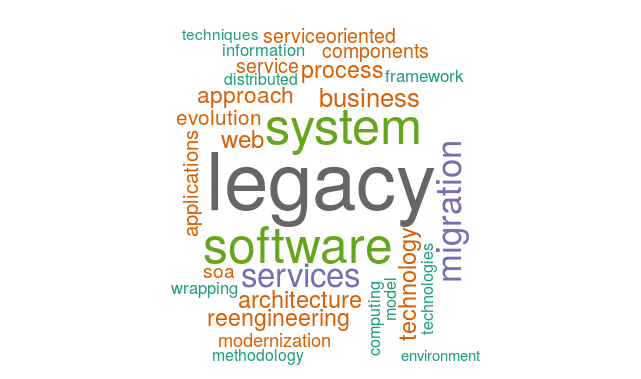
\includegraphics[scale=0.40]{img/mapeamento/word_cloud.png}
\caption{Termos mais citados nos \textit{abstracts} das fontes primárias selecionadas.}
\label{fig:word_cloud}
\end{figure}


\subsection{Análise Relacionada à Segunda Questão de Pesquisa}

Esta questão busca verificar se a abordagem orientada a serviços melhora a qualidade dos produtos de software desenvolvidos no CPD/UnB, a fim de satisfazer as necessidades dos usuários. 
Para isso, faz-se uma análise qualitativa da capacidade de manutenibilidade do novo sistema \acrshort{SAE} a partir da experiência dos participantes do estudo de caso. 

A análise foi realizada em conformidade com a norma de qualidade NBR ISO/IEC 9126-1~\cite{iso2003iec}. Esta norma recomenda que seja definido um \emph{modelo de qualidade} para uma avaliação. Assim, foi definido um modelo de qualidade com base no \emph{modelo de qualidade externa e interna} referido pela norma, como mostra a Figura~\ref{fig:modelo_qualidade}. 


% Modelo de qualidade proposto
%======================================================================================

\begin{figure}[htb]
\centering
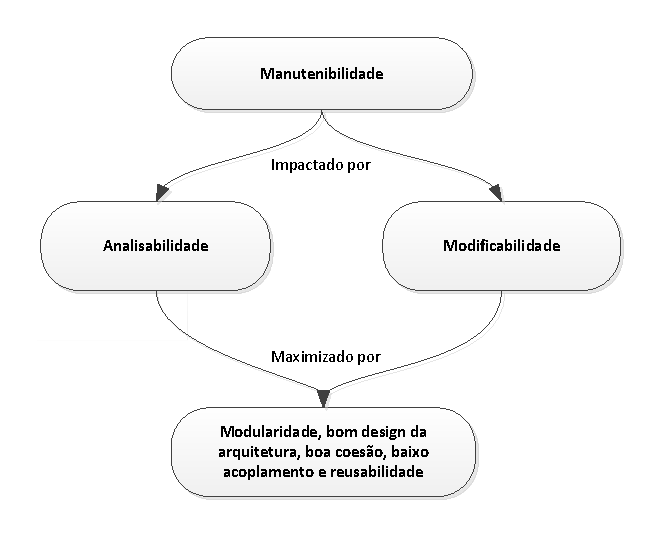
\includegraphics[scale=1]{/img/avaliacao/QP2/modelo_qualidade.pdf}
\caption{Modelo de qualidade proposto para responder a QP2.}
\label{fig:modelo_qualidade}
\end{figure}

O modelo proposto avalia a característica de \emph{manutenibilidade} do
produto de software desenvolvido no estudo de caso (o novo sistema \acrshort{SAE}), 
sendo que foram selecionadas as sub-características da manutenibilidade denominadas
\emph{analisabilidade} e \emph{modificabilidade}, 
as quais servem como uma lista de verificação
de tópicos relacionados com a qualidade avaliada nessa questão. 

A manutenibilidade é uma característica inerente a um produto de software e refere-se a capacidade do mesmo em sofrer correções, melhorias ou adaptações para satisfazerem aos requisitos ou especificações funcionais dos usuários~\cite{iso2003iec, sant2003reuse}. Por definição, a sub-característica analisabilidade compreende a capacidade do produto de software em permitir um diagnóstico das deficiências ou causas de falhas no software, ou a identificação de partes a serem modificadas. Por sua vez, a sub-característica modificabilidade representa a capacidade do produto de software em permitir que uma modificação especificada seja implementada~\cite{iso2003iec}.

É importante salientar, como sugere~\cite{fenton2014software}, que não é possível na prática
medir todas as sub-características internas e externas de um produto
de software, razão pela qual delimitou-se 
nesta investigação as sub-características analisabilidade e modificabilidade
da manutenibilidade, uma vez que o
foco do trabalho de dissertação é propor uma abordagem \acrshort{SOA} 
que seja de fácil manutenção. 

Tradicionalmente, o trabalho de manutenção em um software ocorre após o mesmo entrar em produção e é necessário satisfazer algum requisito ou necessidade que justifique a sua alteração. Para~\cite{S01_bennett2000software}, a manutenção prolonga a vida útil de um software ao mantê-lo atualizado, devendo ser incorporada ao produto de software desde o início de seu desenvolvimento.

Em um primeiro momento, buscou-se verificar a manutenibilidade do sistema \acrshort{SAE}, analisando empiricamente as sub-características analisabilidade e modificabilidade de forma qualitativa. Posteriormente, ao final deste capítulo, será apresentado uma avaliação quantitativa baseada nas métricas propostas por Chidamber \& Kemere~\cite{chidamber1994metrics} para complementar a análise qualitativa, sendo portanto, secundário neste trabalho de dissertação.

De acordo com~\cite{sant2003reuse}, há várias formas de se avaliar a manutenibilidade de um produto de software. Por exemplo, medindo o tempo para aplicar determinada alteração no código fonte ou esforço para diagnosticar determinado problema no software. Também pode-se acompanhar o histórico de modificações de um sistema no repositório de versões desse software. Nesta avaliação, optou-se por mensurar a manutenibilidade por meio da comparação do código fonte do \acrshort{SAE} e outros sistemas da \acrshort{UnB}.

As Figuras~\ref{fig:dependency_diagram_sae_vb},~\ref{fig:dependency_diagram_sae_csharp} 
e~\ref{fig:dependency_diagram_sae_java} mostram três diagramas da arquitetura do \acrshort{SAE} e suas dependências nas versões VB, C\# e Java, respectivamente. Destaca-se que a versão em Java foi desenvolvida durante o estudo de caso com a abordagem proposta neste trabalho de dissertação. Esses diagramas foram produzidos 
utilizando a suíte de ferramentas de análise estática da empresa CodeGear, 
disponível no sítio \url{http://www.codergears.com}. 

Como pode-se observar nos diagramas apresentados, tanto a versão VB quanto a C\# possuem um design monolítico em sua arquitetura. O design monolítico compreende uma das arquiteturas mais comuns e antigas da Engenharia de Software, onde os componentes estão contidos no núcleo do sistema. Nesse \emph{tipo de arquitetura}, como salienta~\cite{clements2002documenting}, a aplicação é composta por vários módulos que são compilados e unidos formando um grande sistema. A maioria dos sistemas em VB e C\# da \acrshort{UnB} segue esta arquitetura, sendo projetados com baixa modularidade e sem qualquer compromisso com o reuso na época em que foram desenvolvidos. 

Segundo o Gestor dos sistemas acadêmicos do CPD/UnB, os principais problemas decorrentes dessa arquitetura, observados nos sistemas legados da \acrshort{UnB}, estão relacionados com a complexidade e o tamanho dos códigos fonte que dificultam a compreensão e a manutenção. Por exemplo, na versão VB do \acrshort{SAE} 
identificou-se um artefato chamado \emph{frmAtzEstSocioEconomico} com aproximadamente 6673 linhas de código. 

Nesse caso, módulos com muitas responsabilidades são difíceis de entender, como é possível presumir, tornando a manutenção muito resistente, passível de erros e comprometendo as propriedades de analisabilidade e modificabilidade. Por conta disso, os desenvolvedores do CPD/UnB, geralmente, evitam alterar os sistemas legados, a não ser quando realmente necessárias.

De modo geral, a única forma de reuso nesses sistemas se dá por meio do acesso ao banco de dados ou através de bibliotecas de funções. Assim, quando necessita-se compartilhar dados ou alguma lógica de negócio, normalmente, criam-se \textit{views} ou \textit{stored procedures} no banco de dados. As bibliotecas de funções contém funções de uso geral e não estão estritamente ligadas as regras de negócios dos sistemas da \acrshort{UnB}. Especificamente, nas aplicações em VB, são muito comuns as regras de negócios estarem na mesma camada onde implementam-se as interfaces com o usuário. Consequentemente, fragmentos de regras de negócios são replicadas em várias telas, dificultando a modificação do software, pois se uma regra mudar, o desenvolvedor precisa revisar o código do sistema para garantir que a lógica foi alterada em todos os locais. 

Por outro lado, até mesmo os sistemas desenvolvidos em Java a partir de 2010
seguem uma arquitetura monolítica com algumas melhorias de design discutidas mais adiante, como 
é o caso do sistema \acrshort{SIGER}, o gerador de relatórios para as aplicações web; o \acrshort{SIEX}, o sistema de informações e extensão; e o \acrshort{SIMAR}, o sistema para gestão das compras de materiais da Universidade. Como curiosidade, o \acrshort{SIMAR} foi migrado parcialmente para Java de acordo com o seu direcionamento estratégico que foi priorizar o módulo de pedidos enquanto que o restante do sistema continuaria funcionando na versão legada. Note que,
sem uma abordagem orientada a serviços, as regras de negócios contidas na versão VB do \acrshort{SIMAR} foram replicadas na versão em Java e, atualmente, a versão Java já contém funcionalidades
não presentes na versão legada, resultado da evolução natural do sistema para atender os 
requisitos dos usuários.


Os sistemas em C\# e Java da \acrshort{UnB} utilizam também uma arquitetura em três camadas para separar a interface com o usuário, o domínio de negócio e a camada de persistência das aplicações. De acordo com a literatura, a arquitetura em camadas auxilia na separação de conceitos e pode trazer ganhos na facilidade de compreensão e na manutenção dos sistemas~\cite{clements2002documenting}. Contudo, o design das aplicações da \acrshort{UnB} continuaram monolíticas, não sendo possível conversarem entre si, a não ser pelo banco de dados. Mesmo com a introdução de bibliotecas compartilhadas para as regras de negócios (introduzido pelo CPD em 2013), ainda era necessário recompilar os sistemas e muitas vezes o desenvolvedor não conseguia reutilizar as bibliotecas devido as dependências circulares existentes. A impossibilidade de reutilizar as regras de negócios de maneira fácil acabou gerando um grande problema para o CPD: a duplicação das classes de negócios entre os sistemas. Assim, os códigos das classes de negócios foram sendo aos poucos replicados entre os sistemas, conforme a necessidade do desenvolvedor. A Figura \ref{fig:duplicidade_usuario_negocio} ilustra esse problema com a classe \emph{UsuarioNegocio} que está replicada em vários sistemas Java. Outro ponto colateral dessas redundâncias, é que muitas classes após serem replicadas, sofrem modificações e começam a evoluir separadamente.

\begin{figure}[ht]
\centering
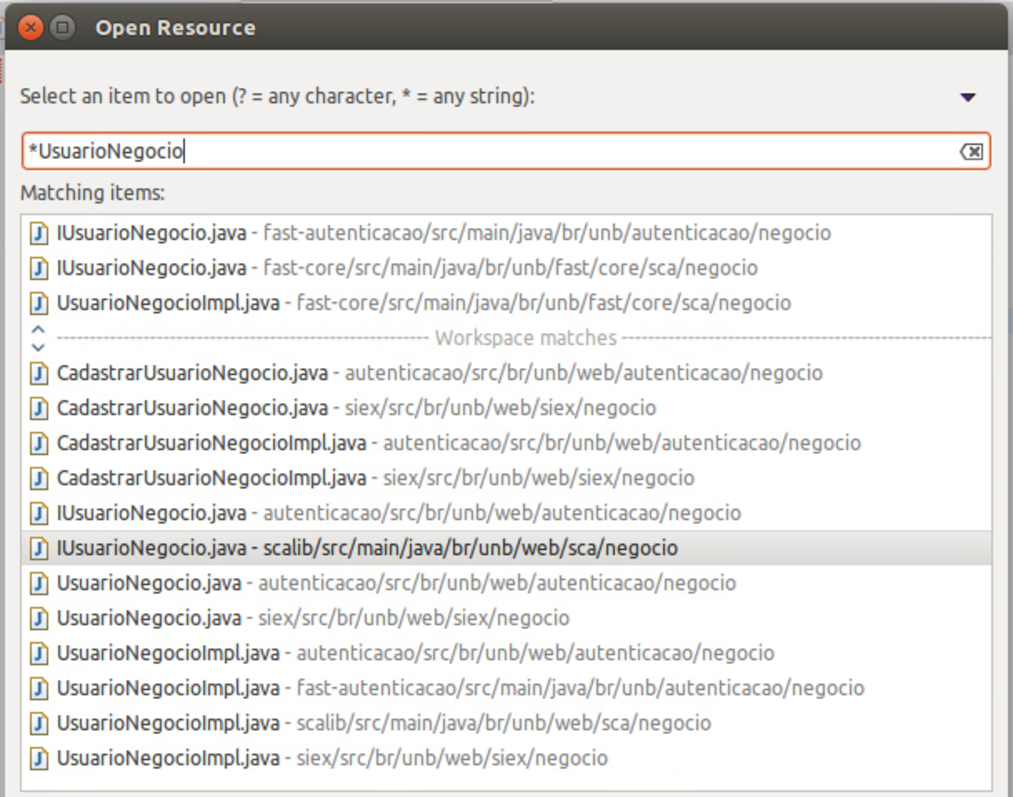
\includegraphics[scale=0.8]{img/avaliacao/QP2/duplicidade_usuario_negocio.pdf}
\caption{Exemplo de classe duplicada entre os sistemas Java.}
\label{fig:duplicidade_usuario_negocio}
\end{figure}

De acordo com o exposto, percebe-se que a manutenibilidade dos sistemas legados da Universidade
(como o \acrshort{SAE} legado) e mesmo os sistemas migrados para Java a partir de 2010,
foram muito impactados pela ausência de modularidade, integração e um bom design arquitetural, tendo como alguns efeitos colaterais observados já discutidos, a duplicidade das regras de negócios, a falta de reuso, a complexidade dos sistemas e o alto custo de manutenção. Assim, possivelmente, uma abordagem SOA aliada a uma boa arquitetura para o desenvolvimento dos serviços poderia minimizar tais problemas.

Nesse aspecto, o último diagrama da Figura~\ref{fig:dependency_diagram_sae_java}, apresenta a arquitetura do novo \acrshort{SAE} usando a arquitetura da abordagem proposta. Uma das preocupações levantadas desde o início dos trabalhos foi a integração lógica das aplicações através de uma camada \acrshort{SOA}, sendo esse papel, realizado pelo barramento e pelo \acrshort{SDK} \emph{ems\_java}, que juntos forneceram uma plataforma \acrshort{SOA} aderente à arquitetura \emph{RESTful} para o projeto. Como é possível notar no diagrama, todos os módulos desenvolvidos na modernização podem compartilhar as suas funcionalidades de forma transparente, bastando invocar os serviços disponíveis no catálogo de serviços do barramento. Salienta-se que o design interno dos módulos auxiliou muito para se chegar nesse objetivo. 

Assim, como discutido na QP1, uma das preocupações dos participantes do estudo de caso foi
empregar um design menos procedimental, razão pela qual decidiu-se utilizar o design \acrshort{DDD}. Este design provê algumas práticas que auxiliam o desenvolvimento de softwares~\cite{evans2004domain}. Uma dessas práticas é a modelagem de domínio do negócio, que promove uma abstração do domínio por meio de um modelo que contempla os aspectos relevantes ao desenvolvimento das aplicações, separando os interesses em domínios de negócios (ou domínios de contextos) separados. Este padrão sugere ainda uma estrutura de objetos que permite que o modelo seja implementado e refletido no código fonte por meio de uma linguagem comum entre as pessoas envolvidas no projeto, seja o especialista no domínio do negócio ou o desenvolvedor~\cite{evans2004domain,vernon2013implementing}. Entre as vantagens indicadas por~\cite{evans2004domain}, está a possibilidade de se obter mais proveito dos benefícios da orientação a objetos, tornando a arquitetura da aplicação mais flexível, fácil de manter e evoluir
com o passar do tempo. 

Nesse sentido, para exemplificar, a Figura~\ref{fig:exemplo_ddd} mostra um exemplo de uma classe Aluno do novo \acrshort{SAE} usando os princípios do \acrshort{DDD}. Foi removido alguns trechos do código fonte original de modo a facilitar a visualização. Como pode-se notar, a classe Aluno possui algumas responsabilidades manifestadas nos métodos declarados nessa classe. Caso fosse utilizado o padrão \textit{Transaction Script}, esta classe não teria nenhum método (objetos anêmicos) e possivelmente as responsabilidades estariam em uma classe de negócio com a classe Aluno servindo meramente como uma estrutura para passar os dados de um aluno entre as camadas do software até a camada de persistência.

\lstset{language=Java,
  basicstyle=\small, %or \small or \footnotesize etc.
  numbersep=10pt,                         % how far the line-numbers are from the code
  tabsize=4,  
  showspaces=false,
  showtabs=false,
  breaklines=true,
  showstringspaces=false,
  breakatwhitespace=true,
  commentstyle=\color{pgreen},
  keywordstyle=\color{pblue},
  stringstyle=\color{pred},
  captionpos=b,
  inputencoding=utf8,
  extendedchars=true,
  literate={á}{{\'a}}1 {ã}{{\~a}}1 {é}{{\'e}}1 {ê}{{\^e}}1 {ç}{{\c{c}}}1 {Ç}{{\c{C}}}1
}
\renewcommand{\lstlistingname}{Código}
\begin{lstlisting}[caption=Exemplo da classe Aluno do sistema SAE, label=fig:exemplo_ddd]
package br.unb.model.sae_context;

public class Aluno {
	private List<OcorrenciaAluno> listaOcorrenciaAluno;

	public void adicionaOcorrenciaAluno(OcorrenciaAluno ocorr){
		if (existeOcorrenciaAberto(ocorr.getSemestreAno(), ocorr.getDataInicio())){
			throw new Exception("O aluno já possui uma ocorrência.");
		}
		
		if (assinouTermoOcorrencia(ocorr.getSemestreAno())){
			throw new Exception("O aluno não possui termo de concessão assinado.");
		}
		
		listaOcorrenciaAluno.add(ocorr);
	}
	
	public List<OcorrenciaAluno> getListaOcorrenciaAluno() {
		return listaOcorrenciaAluno;
	}

	public boolean existeOcorrenciaAberto(String semestreAno, Date dataInicio){
		// Removido para melhor visualização
	}
	
	public boolean assinouTermoOcorrenciaValeAlimentacao(String semestreAno){
		// Removido para melhor visualização
	}
}
\end{lstlisting}





Finalizando a análise da questão QP2, verificaram-se alguns indicativos
qualitativos discutidos que sugerem que a manutenibilidade poderia ser maximizada tanto
pelo processo simplificado da abordagem quanto pela arquitetura
proposta. Porém, alguns desafios identificados durante o estudo de caso
ainda precisam ser melhor investigados para que a abordagem possa ser utilizada. Os 
principais desafios são descritos a seguir:

\begin{itemize}

	\item \textbf{Identificar os serviços que falharam.} A tolerância a falhas não foi o foco deste trabalho mas deverá ser investigado futuramente caso o \acrshort{CPD} opte pela abordagem. Durante os testes, verificou-se que não era possível mapear qual serviço de fato era a origem da falha. Isso pode ser um problema da arquitetura implementada. Por exemplo, quando se introduzia uma falha em um serviço (como o serviço de questionário), vários outros serviços deixavam de funcionar e não era possível identificar que serviço realmente falhou (o que é importante para poder corrigí-lo rapidamente). Seria importante a arquitetura permitir visualizar (se possível) a pilha de chamadas entre os serviços, para verificar qual serviço falhou. Sabe-se que uma das restrições que 
o estilo arquitetural \acrshort{REST} estabelece é que a interação entre 
o cliente e o servidor não deve manter estados entre as comunicações~\cite{fielding2000architectural}. No entanto, a arquitetura da plataforma permite que os serviços comuniquem-se internamente no \textit{cluster} de forma transparente, uma vez que cada serviço é na verdade um processo\footnote{Se o serviço for em Erlang é um processo do ambiente de execução Erlang e, se for em Java é uma \textit{thread} da máquina virtual Java.} que envia/recebe mensagens assíncronas Erlang. Nesse caso, quando um cliente envia uma \emph{requisição REST} para o barramento de serviços e este repassa para o seu destino (o serviço solicitado), a partir daí, as chamadas para outros serviços 
no \textit{cluster} são mensagens Erlang, sendo que nesse caso, poderia haver uma forma de identificar a sequência de chamadas entre os serviços internos para atender a solicitação do cliente, uma vez que todas as chamadas entre os processos passam primeiro pelo processo \emph{Dispatcher} do barramento. 

	\item \textbf{Transformar código procedimental em serviço.}

Este desafio está relacionado as atividades de análise e surgiu devido a dificuldade inerente para transformar código procedural em serviços durante a modernização do \acrshort{SAE}. Note que essa foi uma das atividades identificadas na QP1 mais difíceis de serem realizadas. Em um processo de modernização típico do CPD, que atualmente não é documentado, a migração dos sistemas legados segue o conceito \textit{Transaction Script}, que é relativamente mais direta e fácil de se fazer, uma vez que simplesmente se reescreve o que está no sistema legado para o novo sistema. Não é necessário pensar muito em como fazer, no máximo, vai haver a separação dos códigos de negócios da interface com o usuário e será criado a camada de persistência. Por outro lado, quando se pensa em oferecer serviços reutilizáveis, é necessário pensar na forma como será exposto o serviço, quais os parâmetros de entrada e o que o serviço vai retornar, para que ao final, tenha um bom design da \acrshort{API} e possa ser utilizado pelos clientes.

\end{itemize}


% Diagrama de dependências das três versões do SAE
%======================================================================================


\begin{figure}[htb]
\centering
\includegraphics[scale=0.37]{/img/avaliacao/QP2/metrics/SaeVB/ComponentDependenciesDiagram.png}
\caption{Diagrama de dependências do sistema \acrshort{SAE} na versão VB.}
\label{fig:dependency_diagram_sae_vb}
\end{figure}



\begin{figure}[htb]
\centering
\includegraphics[scale=0.37]{/img/avaliacao/QP2/metrics/SaeWeb/ComponentDependenciesDiagram.png}
\caption{Diagrama de dependências do sistema \acrshort{SAE} na versão C\#.}
\label{fig:dependency_diagram_sae_csharp}
\end{figure}



\begin{figure}[htb]
\centering
\includegraphics[scale=0.4]{/img/avaliacao/QP2/metrics/SaeJava/ComponentDependenciesDiagram.png}
\caption{Diagrama de dependências do sistema \acrshort{SAE} na versão Java.}
\label{fig:dependency_diagram_sae_java}
\end{figure}



\subsection{Análise Quantitativa Complementar}

Além da avaliação qualitativa apresentada anteriormente, optou-se por incluir uma \emph{análise quantitativa complementar} utilizando algumas métricas de software identificadas na literatura~\cite{chidamber1994metrics, fenton2014software, gyimothy2005empirical, mccabe1976complexity}, descritas resumidamente a seguir:

\begin{enumerate}[(M1)]

\item{Line of Code (LoC)}

A métrica LoC é uma métrica tradicional para mensurar o tamanho físico de um software. Calcula-se nessa avaliação o número de linhas de código que cada sistema avaliado contém. Não são contabilizados documentações, comentários para explicar o que o código faz, nem as linhas em branco, segundo as observações de~\cite{fenton2014software}.

\item{Cyclomatic Complexity (CC)}

Métrica para medir a complexidade de um software e consiste basicamente em contar o número de caminhos diferentes que um método pode ter. É obtido através de heurísticas e independe da linguagem de programação.
Segundo o seu criador \emph{McCabe`s}~\cite{mccabe1976complexity}, é uma das métricas mais utilizadas para mensurar a complexidade de softwares (tanto para sistemas orientados a objetos quanto os procedurais).


\item{Weighted Methods Per Class (WMC)}

Mensura a complexidade das classes em termos da soma das complexidades dos métodos. De acordo com ~\cite{chidamber1994metrics}, o número de métodos de uma classe é uma forma efetiva para estimar o tempo e o esforços de manutenção para uma classe.


\item{Coupling Between Objects (CBO)}

Verifica o acoplamento entre objetos, ou seja, o nível de dependências entre as classes. Calcula-se aqui duas variáveis: o \emph{acoplamento eferente} (a quantidade de classes que uma classe depende) e; o \emph{acoplamento aferente} (a quantidade de classes que dependem de uma classe).

\item{Lack of Cohesion of Methods (LCOM)}

Avalia a falta de coesão entre os métodos de uma classe. Representa a diferença entre o número de pares de métodos de uma classe que não compartilham o mesmo conjunto de atributos e o número de pares que compartilham. Existem algumas variações dessa métrica. Nessa avaliação, o algoritmo utilizado é o LCOM1 de Chidamber \& Kemerer~\cite{chidamber1994metrics}.

\end{enumerate}


As métricas foram coletadas com a suíte de análise estática da empresa CoderGears\footnote{A suíte de ferramentas CodeGears está disponível no sítio \url{http://www.codergears.com}.} e com a ferramenta CLOC\footnote{A ferramenta CLOC está disponível no sítio \url{http://cloc.sourceforge.net}.}. Salienta-se que a justificativa para a seleção dessas métricas é verificar quantitativamente se o sistema modernizado no estudo de caso possui indicativos
de uma arquitetura melhor quando comparado com os demais sistemas da UnB, em termos de modularidade, coesão e acoplamento, atributos que podem segundo~\cite{fenton2014software}, contribuir na maximização da manutenibilidade dos sistemas de software. 

Nesse sentido, os sistemas selecionados para a análise estão listados na Tabela~\ref{sistemas_avaliados}. 

% Tabela dos sistemas para a avaliação
%======================================================================================
\begin{table}[!htb]
\centering
\small
\caption{Listagem dos sistemas avaliados.}
\label{sistemas_avaliados}
\begin{tabular}{|
>{\columncolor[HTML]{EFEFEF}}c |l|c|c|c|}
\hline
\cellcolor[HTML]{C0C0C0}\textbf{Sistema} & \multicolumn{1}{c|}{\cellcolor[HTML]{C0C0C0}\textbf{Descrição do Sistema}}                                 & \cellcolor[HTML]{C0C0C0}\textbf{\begin{tabular}[c]{@{}c@{}}Métrica    \\ LoC\end{tabular}} & \cellcolor[HTML]{C0C0C0}\textbf{\begin{tabular}[c]{@{}c@{}}Linguagem de \\ Programação\end{tabular}} & \cellcolor[HTML]{C0C0C0}\textbf{\begin{tabular}[c]{@{}c@{}}Desenvolvido\\ Em\end{tabular}} \\ \hline
\textbf{SAE}                             & Sistema de Estudo Socioeconômico                                                                           & 16087                                                                                      & VB                                                                                                   & 2000                                                                                       \\ \hline
\textbf{SAE}                             & Sistema de Estudo Socioeconômico                                                                           & 11078                                                                                      & C\#                                                                                                  & 2007                                                                                       \\ \hline
\textbf{SITAB}                           & Sistema de Tabelas de Apoio                                                                                & 14453                                                                                      & JAVA                                                                                                 & 2012                                                                                       \\ \hline
\textbf{SIADD}                           & Sistema de Avaliação de Docentes                                                                           & 39101                                                                                      & JAVA                                                                                                 & 2013                                                                                       \\ \hline
\textbf{SICONV}                          & Sistema de Convênios                                                                                       & 3796                                                                                       & JAVA                                                                                                 & 2014                                                                                       \\ \hline
\textbf{SIMAR}                           & Sistema de Materiais                                                                                       & 3213                                                                                       & JAVA                                                                                                 & 2015                                                                                       \\ \hline
\textbf{SAE}                             & \begin{tabular}[c]{@{}l@{}}Sistema de Estudo Socioeconômico\\ desenvolvido no estudo de caso.\end{tabular} & \textbf{9558}                                                                              & JAVA                                                                                                 & \textbf{2015}                                                                              \\ \hline
\end{tabular}
\end{table}



 
A métrica LoC pode ser visualizada na Tabela~\ref{sistemas_avaliados}. A Figura~\ref{fig:proporcao_tam_sae_versoes} mostra também um gráfico com as três versões do \acrshort{SAE}. As demais métricas coletadas estão disponíveis na Tabela~\ref{tab:coleta_metricas_sae}. Destaca-se que a granularidade da métrica LoC é por aplicação e as demais métricas é por classe ou componente (também chamado de \emph{entidade}) para obter mais informações sobre os sistemas e a sua arquitetura correspondente.

De acordo com a Figura~\ref{fig:proporcao_tam_sae_versoes}, as versões VB, C\# e Java do \acrshort{SAE} tem 16087, 11078, 9558 linhas de código respectivamente. A métrica LoC tem um propósito apenas informativo já que cada linguagem tem suas próprias características. Salienta-se que o novo \acrshort{SAE} é dividido em módulos \textit{back-end} (com os serviços de negócios) e o \textit{front-end} da aplicação (que ainda não está completo). O Código fonte completo pode ser consultado no sítio \url{https://github.com/erlangMS/samples/tree/master/sae/backend}.


% Figura que mostra o tamanho de cada versão do SAE
%======================================================================================

\begin{figure}[htb]
\centering
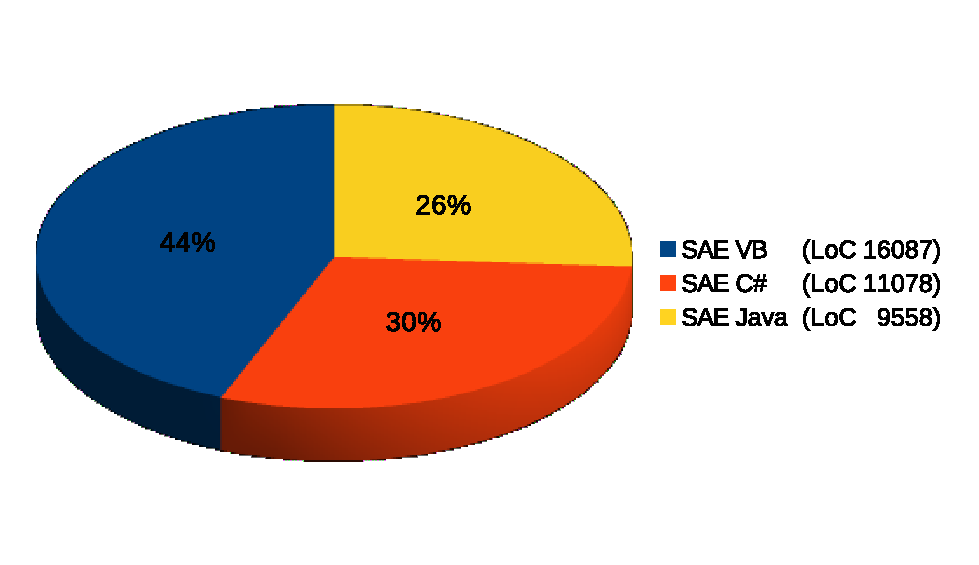
\includegraphics[scale=0.72]{/img/avaliacao/QP2/proporcao_tam_sae_versoes.eps}
\caption{Métrica LoC nas três versões do SAE.}
\label{fig:proporcao_tam_sae_versoes}
\end{figure}


Examinando a métrica WMC, percebe-se que os sistemas diferem nesse quesito. Tome como exemplo o \acrshort{SAE} Java com média WMC=8,17 em comparação ao \acrshort{SAE} VB com WMC=14,05 e o \acrshort{SAE} C\# com WMC=12,55. Segundo~\cite{chidamber1994metrics}, um valor médio até 10 é considerado bom e a partir disso, o sistema pode apresentar certa dificuldade em sua manutenção. Como se observa, a maior parte dos sistemas estão acima desse indicador ou apresentam alguma entidade acima deste valor, como indica a medição Max. Apenas como curiosidade, descobriu-se uma classe chamada \emph{VoEstudosSocioEconomicos} em C\# com 171 atributos, a qual os participantes decidiram refatorar em várias classes menores.

Analisando a complexidade ciclomática (métrica CC), verificou-se que o novo \acrshort{SAE} é muito parecido com o \acrshort{SAE} C\#. Segundo afirma~\cite{watson1996structured}, um valor até 10 é considerado bom e há boas razões para limitar essa complexidade ciclomática. Por exemplo, artefatos muito complexos são alvo de mais problemas, são difíceis entendê-los, testá-los e modificá-los. De acordo com esse limite, os sistemas \acrshort{SIADD}, \acrshort{SICONV} e o \acrshort{SIMAR}, provavelmente, precisariam ser revistos já que a complexidade ciclomática média foi ultrapassada. Todos os sistemas analisados tem alguma entidade que ultrapassou este limite, como por exemplo, o \acrshort{SIADD} com Max=322, o \acrshort{SICONV} com Max=109 e o \acrshort{SIMAR} com Max=123. 

Além disso, comparando os dados coletados da métrica LCOM, que mede a falta de coesão entre os métodos de uma classe, pode-se notar que o novo \acrshort{SAE} é o sistema mais coeso da lista. Para o \acrshort{SAE} C\#, foi pontuado o valor 0 para todas as entidades, podendo ser um erro ou limitação da ferramenta de análise estática na linguagem C\#. O princípio básico desta métrica é que as classes não devem ter muitas responsabilidades, limitando este valor na faixa entre 0 até 1. Valores altos apontam classes geralmente pouco coesas, como afirmam~\cite{chidamber1994metrics, gyimothy2005empirical}. Acredita-se que o design \acrshort{DDD} pode ter favorecido uma boa pontuação para o \acrshort{SAE} Java.

Do modo geral, o resultado obtido analisando as métricas de software 
nos sistemas selecionados indica que o novo sistema \acrshort{SAE} apresenta alguns
indicativos de uma melhora arquitetural, uma vez que as médias (Avg) e o desvio padrão (Std.) 
apontadas nas métricas coletadas são um pouco melhores no \acrshort{SAE} que nos
demais sistemas avaliados. No entanto, apenas com uma \emph{análise quantitativa}
não foi possível afirmar que a manutenibilidade poderia ser maximizada com 
o uso da abordagem proposta.


% Tabela de estatisticas coletadas
%======================================================================================
\begin{table}[!htb]
\centering
\caption{Coleta de estatísticas dos sistemas avaliados.}
\label{tab:coleta_metricas_sae}
\begin{tabular}{|c|c|c|c|c|c|c|}
\hline
\rowcolor[HTML]{C0C0C0} 
\cellcolor[HTML]{C0C0C0}                                                                                                      & \cellcolor[HTML]{C0C0C0}                                                                                     & \cellcolor[HTML]{C0C0C0}                                   & \multicolumn{4}{c|}{\cellcolor[HTML]{C0C0C0}\textbf{Estatísticas}}                             \\ \cline{4-7} 
\multirow{-2}{*}{\cellcolor[HTML]{C0C0C0}\textbf{\begin{tabular}[c]{@{}c@{}}Sistema / \\ Linguagem\end{tabular}}}             & \multirow{-2}{*}{\cellcolor[HTML]{C0C0C0}\textbf{\begin{tabular}[c]{@{}c@{}}Desenvolvido\\ em\end{tabular}}} & \multirow{-2}{*}{\cellcolor[HTML]{C0C0C0}\textbf{Métrica}} & \textit{\textbf{Avg}} & \textit{\textbf{Max}} & \textit{\textbf{Min}} & \textit{\textbf{Std.}} \\ \hline
\rowcolor[HTML]{EFEFEF} 
\cellcolor[HTML]{EFEFEF}{\color[HTML]{000000} }                                                                               & \cellcolor[HTML]{FFFFFF}                                                                                     & \textbf{CC}                                                & 7,10                  & 39,16                 & 0                     & 10,25                  \\ \cline{3-7} 
\cellcolor[HTML]{EFEFEF}{\color[HTML]{000000} }                                                                               & \cellcolor[HTML]{FFFFFF}                                                                                     & \textbf{WMC}                                               & 14,08                 & 65                    & 1                     & 13,84                  \\ \cline{3-7} 
\rowcolor[HTML]{EFEFEF} 
\cellcolor[HTML]{EFEFEF}{\color[HTML]{000000} }                                                                               & \cellcolor[HTML]{FFFFFF}                                                                                     & \textbf{LCOM}                                              & 0,85                  & 1                     & 0                     & 0,16                   \\ \cline{3-7} 
\rowcolor[HTML]{EFEFEF} 
\cellcolor[HTML]{EFEFEF}{\color[HTML]{000000} }                                                                               & \cellcolor[HTML]{FFFFFF}                                                                                     & \textbf{AC}                                                & 78,81                 & 1854                  & 0                     & 286,84                 \\ \cline{3-7} 
\multirow{-5}{*}{\cellcolor[HTML]{EFEFEF}{\color[HTML]{000000} \textbf{\begin{tabular}[c]{@{}c@{}}SAE \\ (VB)\end{tabular}}}} & \multirow{-5}{*}{\cellcolor[HTML]{FFFFFF}\textbf{2000}}                                                      & \textbf{EC}                                                & -                     & -                     & -                     & -                      \\ \hline
\rowcolor[HTML]{EFEFEF} 
\cellcolor[HTML]{EFEFEF}                                                                                                      & \cellcolor[HTML]{FFFFFF}                                                                                     & \textbf{CC}                                                & 3,78                  & 20                    & 1                     & 4,87                   \\ \cline{3-7} 
\cellcolor[HTML]{EFEFEF}                                                                                                      & \cellcolor[HTML]{FFFFFF}                                                                                     & \textbf{WMC}                                               & 12,55                 & 171                   & 1                     & 33,33                  \\ \cline{3-7} 
\rowcolor[HTML]{EFEFEF} 
\cellcolor[HTML]{EFEFEF}                                                                                                      & \cellcolor[HTML]{FFFFFF}                                                                                     & \textbf{LCOM}                                              & 0                     & 0                     & 0                     & 0                      \\ \cline{3-7} 
\rowcolor[HTML]{EFEFEF} 
\cellcolor[HTML]{EFEFEF}                                                                                                      & \cellcolor[HTML]{FFFFFF}                                                                                     & \textbf{AC}                                                & 0,54                  & 1                     & 0                     & 0,49                   \\ \cline{3-7} 
\multirow{-5}{*}{\cellcolor[HTML]{EFEFEF}\textbf{\begin{tabular}[c]{@{}c@{}}SAE WEB\\ (C\#)\end{tabular}}}                    & \multirow{-5}{*}{\cellcolor[HTML]{FFFFFF}\textbf{2007}}                                                      & \textbf{EC}                                                & 10,49                 & 25                    & 2                     & 5,31                   \\ \hline
\rowcolor[HTML]{EFEFEF} 
\cellcolor[HTML]{EFEFEF}                                                                                                      & \cellcolor[HTML]{FFFFFF}                                                                                     & \textbf{CC}                                                & 9,26                  & 153                   & 0                     & 12,66                  \\ \cline{3-7} 
\cellcolor[HTML]{EFEFEF}                                                                                                      & \cellcolor[HTML]{FFFFFF}                                                                                     & \textbf{WMC}                                               & 6,07                  & 93                    & 0                     & 7,02                   \\ \cline{3-7} 
\rowcolor[HTML]{EFEFEF} 
\cellcolor[HTML]{EFEFEF}                                                                                                      & \cellcolor[HTML]{FFFFFF}                                                                                     & \textbf{LCOM}                                              & 0,58                  & 1                     & 0                     & 0,37                   \\ \cline{3-7} 
\rowcolor[HTML]{EFEFEF} 
\cellcolor[HTML]{EFEFEF}                                                                                                      & \cellcolor[HTML]{FFFFFF}                                                                                     & \textbf{AC}                                                & 1,62                  & 48                    & 0                     & 4,13                   \\ \cline{3-7} 
\multirow{-5}{*}{\cellcolor[HTML]{EFEFEF}\textbf{\begin{tabular}[c]{@{}c@{}}SITAB WEB\\ (JAVA)\end{tabular}}}                 & \multirow{-5}{*}{\cellcolor[HTML]{FFFFFF}\textbf{2012}}                                                      & \textbf{EC}                                                & 8,71                  & 27                    & 0                     & 4,41                   \\ \hline
\rowcolor[HTML]{EFEFEF} 
\cellcolor[HTML]{EFEFEF}                                                                                                      & \cellcolor[HTML]{FFFFFF}                                                                                     & \textbf{CC}                                                & 19,89                 & 322                   & 0                     & 25,72                  \\ \cline{3-7} 
\cellcolor[HTML]{EFEFEF}                                                                                                      & \cellcolor[HTML]{FFFFFF}                                                                                     & \textbf{WMC}                                               & 16,66                 & 322                   & 0                     & 19,07                  \\ \cline{3-7} 
\rowcolor[HTML]{EFEFEF} 
\cellcolor[HTML]{EFEFEF}                                                                                                      & \cellcolor[HTML]{FFFFFF}                                                                                     & \textbf{LCOM}                                              & 0,79                  & 1                     & 0                     & 0,21                   \\ \cline{3-7} 
\rowcolor[HTML]{EFEFEF} 
\cellcolor[HTML]{EFEFEF}                                                                                                      & \cellcolor[HTML]{FFFFFF}                                                                                     & \textbf{AC}                                                & 3,53                  & 84                    & 0                     & 8,27                   \\ \cline{3-7} 
\multirow{-5}{*}{\cellcolor[HTML]{EFEFEF}\textbf{\begin{tabular}[c]{@{}c@{}}SIADD WEB\\ (JAVA)\end{tabular}}}                 & \multirow{-5}{*}{\cellcolor[HTML]{FFFFFF}\textbf{2013}}                                                      & \textbf{EC}                                                & 11,32                 & 323                   & 0                     & 17,16                  \\ \hline
\rowcolor[HTML]{EFEFEF} 
\cellcolor[HTML]{EFEFEF}                                                                                                      & \cellcolor[HTML]{FFFFFF}                                                                                     & \textbf{CC}                                                & 12,56                 & 109                   & 0                     & 19,87                  \\ \cline{3-7} 
\cellcolor[HTML]{EFEFEF}                                                                                                      & \cellcolor[HTML]{FFFFFF}                                                                                     & \textbf{WMC}                                               & 7,73                  & 71                    & 0                     & 11,11                  \\ \cline{3-7} 
\rowcolor[HTML]{EFEFEF} 
\cellcolor[HTML]{EFEFEF}                                                                                                      & \cellcolor[HTML]{FFFFFF}                                                                                     & \textbf{LCOM}                                              & 0,57                  & 1                     & 0                     & 0,36                   \\ \cline{3-7} 
\rowcolor[HTML]{EFEFEF} 
\cellcolor[HTML]{EFEFEF}                                                                                                      & \cellcolor[HTML]{FFFFFF}                                                                                     & \textbf{AC}                                                & 2,12                  & 32                    & 0                     & 4,68                   \\ \cline{3-7} 
\multirow{-5}{*}{\cellcolor[HTML]{EFEFEF}\textbf{\begin{tabular}[c]{@{}c@{}}SICONV WEB\\ (JAVA)\end{tabular}}}                & \multirow{-5}{*}{\cellcolor[HTML]{FFFFFF}\textbf{2014}}                                                      & \textbf{EC}                                                & 9,27                  & 35                    & 0                     & 7,25                   \\ \hline
\rowcolor[HTML]{EFEFEF} 
\cellcolor[HTML]{EFEFEF}                                                                                                      & \cellcolor[HTML]{FFFFFF}                                                                                     & \textbf{CC}                                                & 13,75                 & 123                   & 0                     & 24,83                  \\ \cline{3-7} 
\cellcolor[HTML]{EFEFEF}                                                                                                      & \cellcolor[HTML]{FFFFFF}                                                                                     & \textbf{WMC}                                               & 10,52                 & 68                    & 0                     & 15,80                  \\ \cline{3-7} 
\rowcolor[HTML]{EFEFEF} 
\cellcolor[HTML]{EFEFEF}                                                                                                      & \cellcolor[HTML]{FFFFFF}                                                                                     & \textbf{LCOM}                                              & 0,52                  & 1                     & 0                     & 0,34                   \\ \cline{3-7} 
\rowcolor[HTML]{EFEFEF} 
\cellcolor[HTML]{EFEFEF}                                                                                                      & \cellcolor[HTML]{FFFFFF}                                                                                     & \textbf{AC}                                                & 1,54                  & 13                    & 0                     & 2,82                   \\ \cline{3-7} 
\multirow{-5}{*}{\cellcolor[HTML]{EFEFEF}\textbf{\begin{tabular}[c]{@{}c@{}}SIMAR WEB\\ (JAVA)\end{tabular}}}                 & \multirow{-5}{*}{\cellcolor[HTML]{FFFFFF}\textbf{2015}}                                                      & \textbf{EC}                                                & 8,94                  & 39                    & 0                     & 8,00                   \\ \hline
\rowcolor[HTML]{EFEFEF} 
\cellcolor[HTML]{EFEFEF}                                                                                                      & \cellcolor[HTML]{FFFFFF}                                                                                     & \textbf{CC}                                                & 7,38                  & 42                    & 0                     & 7,08                   \\ \cline{3-7} 
\cellcolor[HTML]{EFEFEF}                                                                                                      & \cellcolor[HTML]{FFFFFF}                                                                                     & \textbf{WMC}                                               & 8,17                  & 32                    & 0                     & 5,65                   \\ \cline{3-7} 
\rowcolor[HTML]{EFEFEF} 
\cellcolor[HTML]{EFEFEF}                                                                                                      & \cellcolor[HTML]{FFFFFF}                                                                                     & \textbf{LCOM}                                              & 0,38                  & 1                     & 0                     & 0,40                   \\ \cline{3-7} 
\rowcolor[HTML]{EFEFEF} 
\cellcolor[HTML]{EFEFEF}                                                                                                      & \cellcolor[HTML]{FFFFFF}                                                                                     & \textbf{AC}                                                & 2,50                  & 16                    & 0                     & 2,58                   \\ \cline{3-7} 
\multirow{-5}{*}{\cellcolor[HTML]{EFEFEF}\textbf{\begin{tabular}[c]{@{}c@{}}SAE WEB\\ (JAVA)\end{tabular}}}                   & \multirow{-5}{*}{\cellcolor[HTML]{FFFFFF}\textbf{2015}}                                                      & \textbf{EC}                                                & 9,44                  & 23                    & 1                     & 4,49                   \\ \hline
\end{tabular}
\end{table}









\section{Ameaças à Validade}\label{ava:ameacas}

A avaliação empírica apresentada limitou-se em avaliar
a aplicação da abordagem proposta 
neste trabalho de dissertação na
modernização de um sistema legado no CPD/UnB, no
contexto da manutenção de software. 

Os participantes do estudo de caso demonstraram muito
interesse em aplicar um abordagem \acrshort{SOA}
na modernização de um sistema legado da \acrlong{UnB}. Com base 
nesses aspectos,
as possíveis ameaças identificadas no estudo, de acordo com
as recomendações de~\cite{kitchenham:2004}, são descritas a seguir:

\begin{itemize}

	\item Validade Interna. Capacidade de um novo experimento repetir o
comportamento atual com os mesmos objetivos. Identificou-se que que
deveria haver um número mínimo de participantes. O estudo de caso
teve 12 participantes, um número que se mostrou adequado para os fins do estudo.

	\item Validade externa. Generalizar os efeitos observados
fora do estudo. Identificou-se que o perfil dos participantes
foi representativo, pois haviam profissionais de alguns outros
órgãos públicos além do CPD/UnB, bem como alunos de graduação
e mestrado da \acrshort{UnB}.

	\item Validade de conclusão. Refere-se à habilidade de se
chegar a uma conclusão. Foi utilizado questionários e métricas
de software para conduzir o experimento e se chegar a uma conclusão.

\end{itemize}

Sabe-se que uma avaliação pode requerer um longo período
para se observar e examinar todas as causas e efeitos do universo
estudado. Para conduzir a avaliação da melhor forma possível, as
atividades foram documentadas em áudio. Além do mais,
devido ao curto período de tempo disponível para o estudo de
caso (apenas 4 meses), optou-se pelo método Pesquisa-Ação que se
mostrou muito conveniente e estabeleceu uma ampla atuação dos
participantes da situação problema (a modernização do \acrshort{SAE}
através da abordagem proposta) de modo cooperativo e participativo. 







